\documentclass[12pt]{article}
    % \usepackage{polski}
    \usepackage[utf8]{inputenc}
    
    \usepackage{lingmacros}
    \usepackage{tree-dvips}
    \usepackage{blindtext}
    \usepackage{graphicx}
    \usepackage{todonotes}
    
    \graphicspath{ {imgs/} }
    
    
    \setcounter{secnumdepth}{0}
    \pagenumbering{gobble}
    
    % \usepackage[top=0.1in, bottom=0.7in, left=1.35in, right=1.35in]{geometry}
    
    \title{Lifelong Learning With Dynamically Expandable Networks -- Reproducibility Report }
    \author{Błażej Sowa, Łukasz Siudek}
    \date{}
    
    \begin{document}
    \maketitle
    
    \section {Motivation}
    
    Lifelong learning (Thrun, 1995), the problem of continual learning where tasks arrive in sequence, is
    an important topic in transfer learning. The primary goal of lifelong learning is to leverage knowledge
    from earlier tasks for obtaining better performance, or faster convergence/training speed on models
    for later tasks. While there exist many different approaches to tackle this problem, we consider
    lifelong learning under deep learning to exploit the power of deep neural networks. Fortunately, for
    deep learning, storing and transferring knowledge can be done in a straightforward manner through
    the learned network weights. The learned weights can serve as the knowledge for the existing tasks,
    and the new task can leverage this by simply sharing these weights.
    
    \section{Introduction}
    
    In this report we are going to show our results of attempted reproduction of a
    recent conference paper from ICLR, called "Lifelong Learning With Dynamically
    Expandable Networks" which proposes a novel deep neural network for lifelong learning, called "Dynamically
    Expandable Network". It performs partial retraining of the network trained on old tasks by exploiting task
    relatedness, while increasing its capacity when necessary to account for new knowledge required
    to account for new tasks, to find the optimal capacity for itself, while also effectively preventing
    semantic drift.
    
    \section {Reproducibility}
    
    \subsection {Available Information Overview}
    
    In this section, we list important reproducibility metrics.  
    
    \subsubsection{Dataset}
    % Information about the location and the retrieval process of the dataset is needed to
    % ensure access to the dataset as used in the study.
    We use the same datasets as those used in the paper.
    \begin{enumerate}  
        \item CIFAR-100 
        \item MNIST-Variation 
    \end{enumerate}
    
    \subsubsection{Data preprocessing}
    % The process of ridding the input data of noise and encoding it into a
    % format acceptable to the learning algorithm. Explicit preprocessing information is the first
    % step towards a successful reproduction exercise. An independent researcher should be able
    % to follow and repeat how the data was preprocessed in the study. Also, it will be useful to
    % find preprocessing output information to compare to e.g. final feature vector dimension
    \todo[inline]{TODO: Z jakiego preprocessingu korzystamy?}
    
    \subsubsection{Dataset Partitions}
    %  Details of how the dataset was divided for use as training and test data.
    For the MNIST dataset, the authors of DEN paper use 1,000/200/5,000 images for train/val/test split for each class.
    They form each task to be one-versus-rest binary classification.
    \todo[inline]{TODO: Jak my dzielimy datasety?}
    
    \subsubsection{Model training}
    % The process of fitting the model to the data. Making available, as much
    % information as possible regarding every decision made during this process is particularly
    % crucial to reproduction. Necessary information include but not limited to:
    % 1. Study parameters
    % 2. Proposed technique details – codes, algorithms etc. (if applicable)
    
    \subsubsection{Model Assessment}
    % Measuring the performance of the model trained in 2. Similar information
    % as in 2 applies here as well.
    
    \subsubsection{Randomization control}
    % Most operations of machine learning algorithms involves randomization.
    % Therefore, it is essential to set seed values to control the randomization process in
    % order to be able to repeat the same process again.
    
    \subsubsection{Software Environment}
    % Due to the fact that software packages/modules are in continual
    % development with possible alterations to internal implementation algorithms, it is important
    % that the details of the software environment used (modules, packages and version numbers)
    % be made available
    
    \subsubsection{Hardware Environment}
    % Some data intensive studies are only
    % reproducible on the same machine capacity as was used to produce the original result. So,
    % the hardware information are sometimes essential.
    
    \subsection {Results}
    
    The following image does not show any wombats
    \includegraphics[height=\baselineskip]{example-image}.
      
    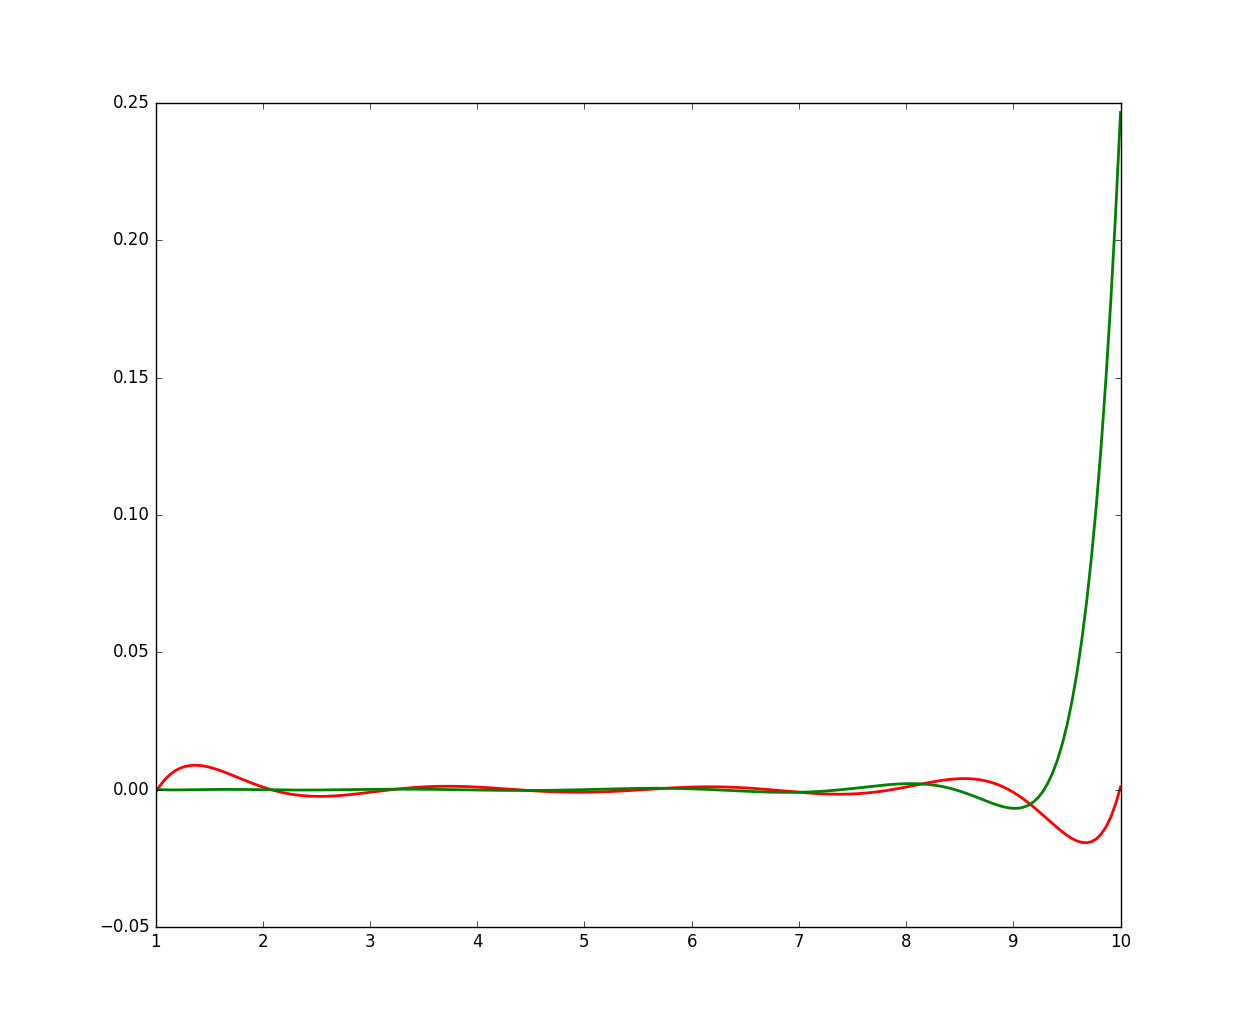
\includegraphics[height=3cm]{figure_1.png}
    
    \includegraphics[height=3cm]{example-image-a} \includegraphics[width=5cm]{example-image-b}
    
    \section {Conclusion}
    
    Conclusion.
    
    % Zawartość sceny do wyrenderowania znajduje się w pliku \texttt{scene.ml}.
    
    \begin{thebibliography}{9}
        \bibitem{lamport94}
            Leslie Lamport,
            \textit{\LaTeX: a document preparation system},
            Addison Wesley, Massachusetts,
            2nd edition,
            1994.
    \end{thebibliography}
    
    \end{document}
        